\documentclass{article}
\usepackage[ansinew]{inputenc} % ASCII (Western Windows CP1252)
\usepackage{tikz}
\usepackage{graphicx}
\usepackage{color}
\usepackage[colorlinks]{hyperref}

\begin{document}

\section{Graphics Inclusion}

\emph{Graphic inclusion in TeX documents is not a WinEdt-related issue. You
should consult the documentation that comes with your TeX System (eg.
graphicx package). Below are a few examples that show that it can be done! It
works with my (default) version of MiKTeX 2.9. However, these examples come
with no guarantee and no support from WinEdt Team. If you are experiencing a
problem with these images then the problem has nothing to do with WinEdt but
rather than your TeX System or Ghostscript.}

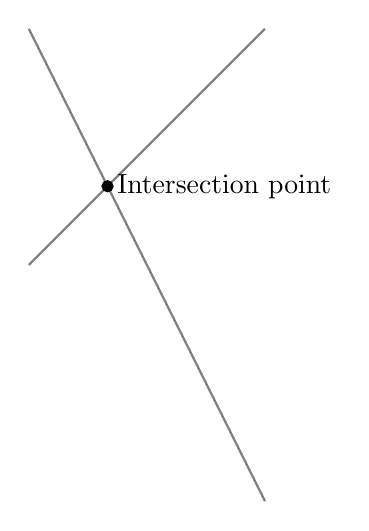
\begin{tikzpicture}
\draw[gray, thick] (-1,2) -- (2,-4);
\draw[gray, thick] (-1,-1) -- (2,2);
\filldraw[black] (0,0) circle (2pt) node[anchor=west] {Intersection point};
\end{tikzpicture}

\end{document}
